\section{Discussion}
\label{discussion}


While Section~\ref{ex_and_re}  demonstrated the significant energy efficiency advantages of the CGLA-based approach, it also highlighted performance bottlenecks under specific conditions. 
To provide architectural insight and guide future work, this section analyzes these limitations from three perspectives: the impact of internal memory size, a granular breakdown of execution phase timings, and the inherent scalability limits imposed by the host system.
\subsection{Impact of LMM Size}
The size of the LMM in each PE is a key architectural design parameter.
This choice directly impacts overall system efficiency, as the LMM capacity governs the fundamental trade-off between performance and power consumption. 
In this subsection, we quantitatively validate our selection of a size of \SI{64}{K\byte} for the LMM, demonstrating that it provides a suitable balance between offload ratio and power efficiency for our target workloads.





In general, increasing the LMM size allows more computational kernels to reside entirely within on-chip memory. 
This strategy tends to improve the offload ratio, which is the proportion of operations executed on the IMAX accelerator rather than the host CPU, thereby reducing overall processing time. 
However, a larger LMM also linearly increases static power consumption, meaning that it does not automatically translate to better energy efficiency. 
Fig.~\ref{fig:PDP_vs_LMM_matrix} clearly illustrates this trade-off. 
For most workloads, increasing the LMM size beyond \SI{64}{K\byte} results in a higher PDP, as the penalty from increased power consumption outweighs the benefit of reduced execution time.
The offload ratios in Table~\ref{tab:model_scores_multirow} explain this phenomenon. 
For most models, a \SI{64}{K\byte} LMM is sufficient to achieve high offload ratios exceeding \SI{85}{\percent}, with the common FP16 kernel fitting entirely within this memory. 
This indicates that at \SI{64}{K\byte}, most targeted computations are already on-chip, offering limited potential for further improvement.
Consequently, the marginal performance improvement from larger LMMs fails to offset their increased power draw, leading to a degradation in PDP, making it more energy-efficient to execute it on the host.
The Qwen3-8B Q8\_0 model, while initially appearing to be an exception, reinforces this conclusion because the substantial size of its Q8\_0 kernel leads to excessive DMA transfer latency.
Consequently, offloading this kernel results in a higher PDP, as the overhead from data transfer outweighs the computational gains.
The most energy-efficient strategy, therefore, is to avoid offloading this specific kernel. 
This is precisely the behavior that a \SI{64}{K\byte} LMM enforces, making it an effective choice even for this challenging case.




\begin{figure}[t]
  \centering
  \subfloat[Qwen3-0.6B Q3\_K\_S\label{fig:sub_a}]{%
    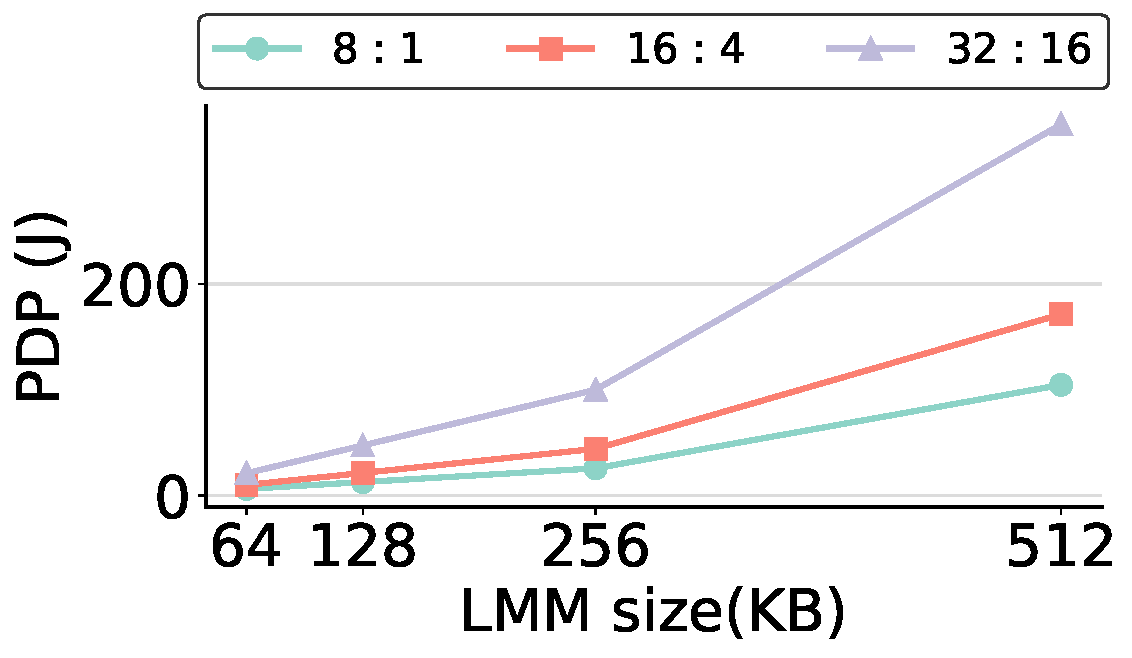
\includegraphics[width=0.23\textwidth]{./PDP_vs_LMM_Qwen3-0.6B_Q3_K_S.pdf}
  }\hspace{0.2em}
  \subfloat[Qwen3-0.6B Q8\_0\label{fig:sub_b}]{%
    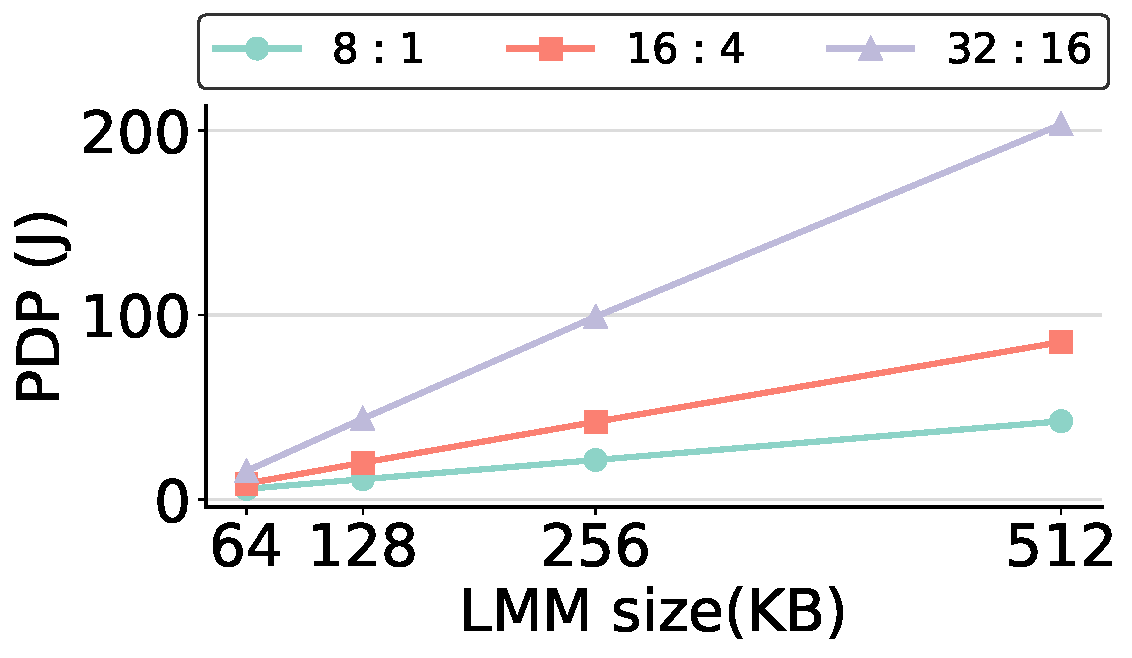
\includegraphics[width=0.23\textwidth]{./PDP_vs_LMM_Qwen3-0.6B_Q8_0.pdf}
  }\par\vspace{1em}
  \subfloat[Qwen3-1.7B Q3\_K\_S\label{fig:sub_c}]{%
    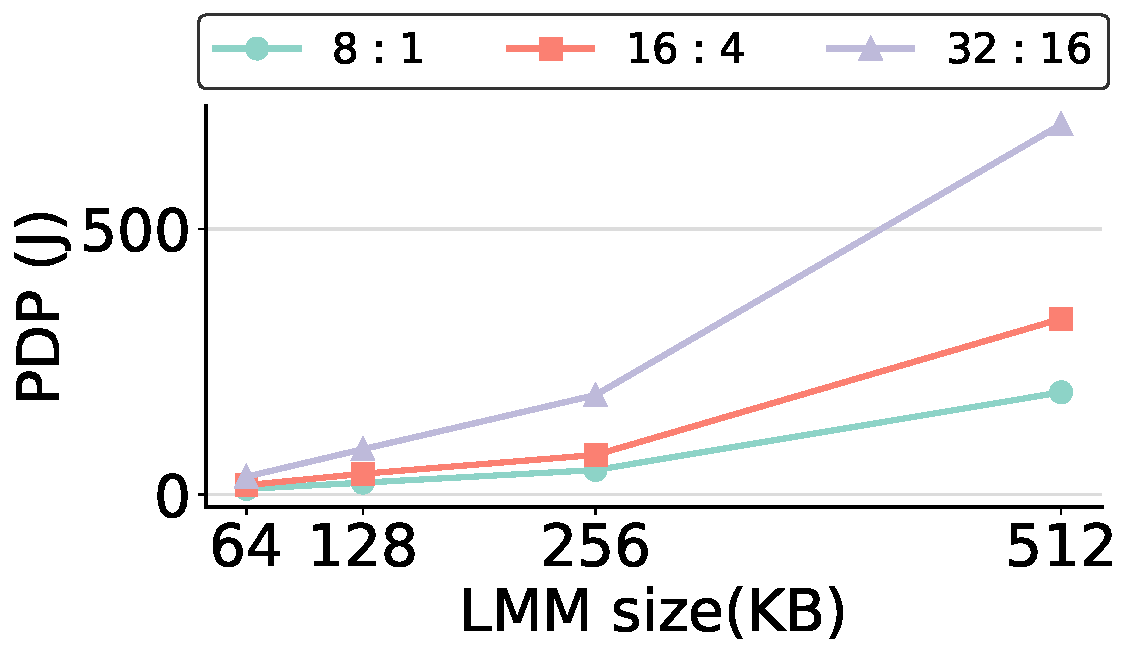
\includegraphics[width=0.23\textwidth]{./PDP_vs_LMM_Qwen3-1.7B_Q3_K_S.pdf}
  }\hspace{0.2em}
  \subfloat[Qwen3-1.7B Q8\_0\label{fig:sub_d}]{%
    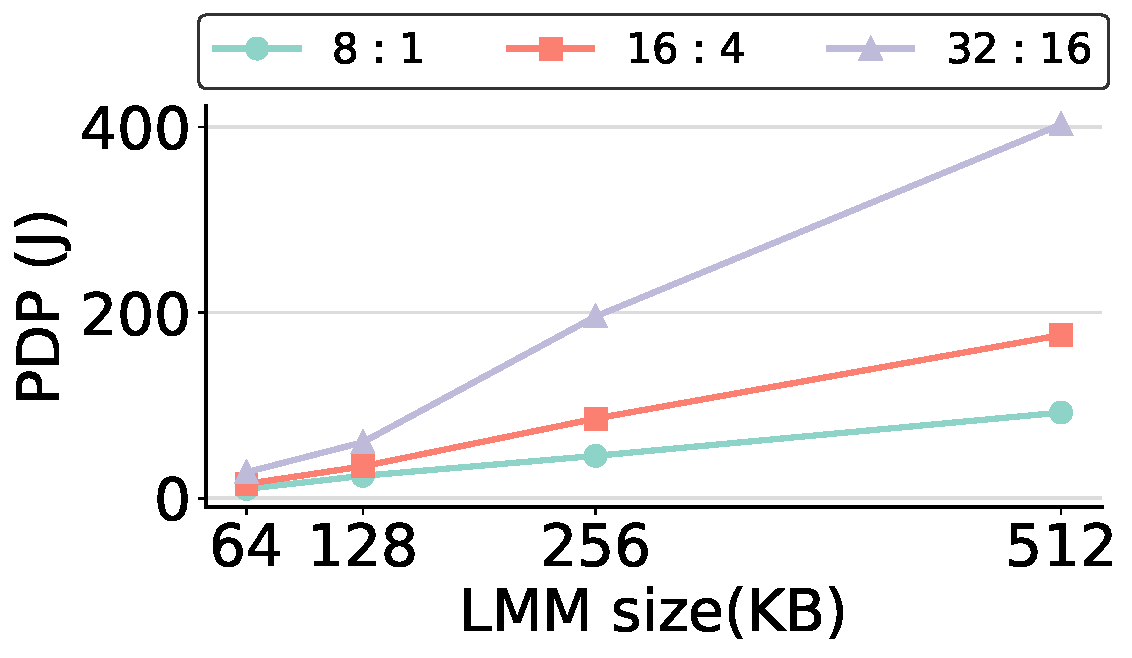
\includegraphics[width=0.23\textwidth]{./PDP_vs_LMM_Qwen3-1.7B_Q8_0.pdf}
  }\par\vspace{1em}
  \subfloat[Qwen3-8B Q3\_K\_S\label{fig:sub_e}]{%
    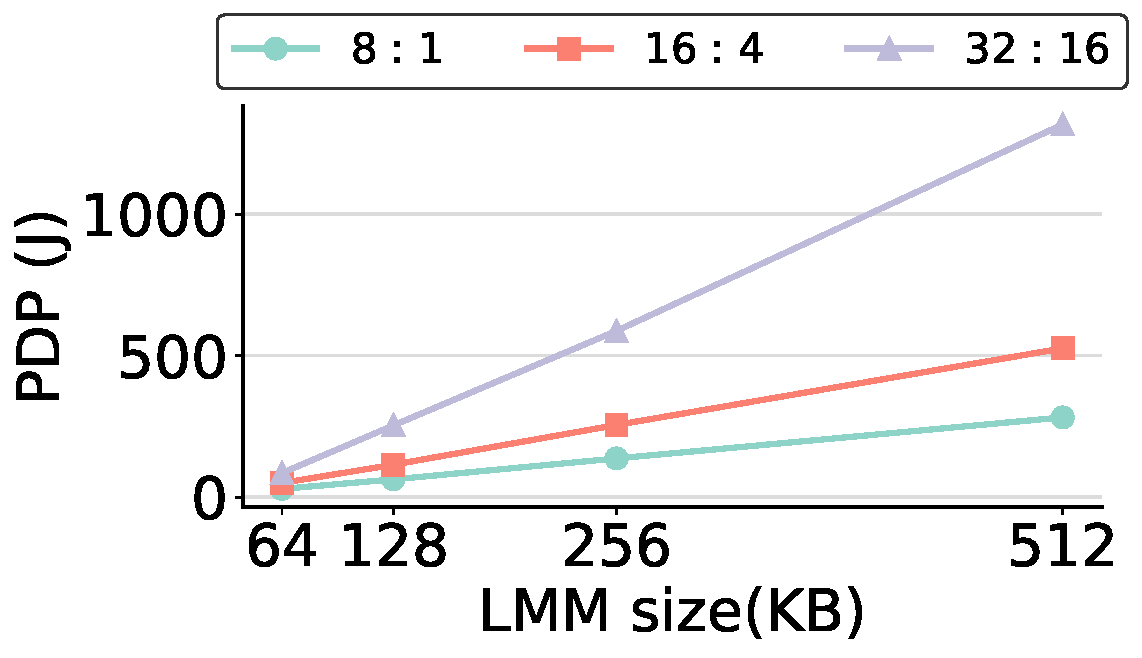
\includegraphics[width=0.23\textwidth]{./PDP_vs_LMM_Qwen3-8B_Q3_K_S.pdf}
  }\hspace{0.2em}
  \subfloat[Qwen3-8B Q8\_0\label{fig:sub_f}]{%
    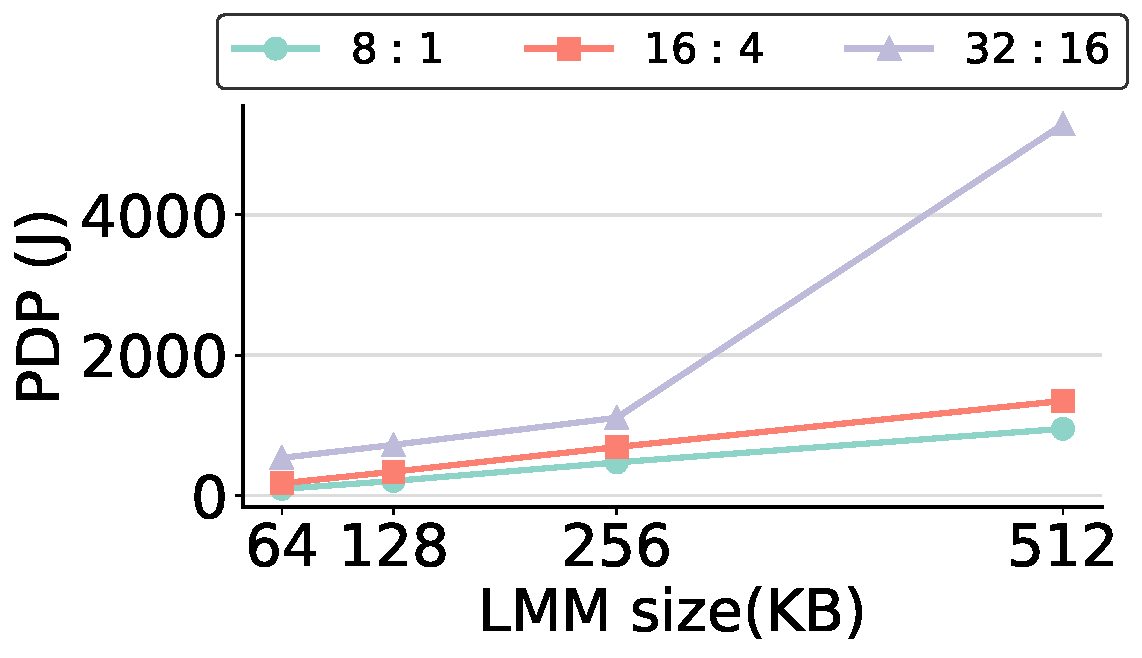
\includegraphics[width=0.23\textwidth]{./PDP_vs_LMM_Qwen3-8B_Q8_0.pdf}
  }
  \caption{Analysis of the impact of LMM size on energy efficiency (PDP, lower is better).}
  \label{fig:PDP_vs_LMM_matrix}
\end{figure}


\begin{table}[t]
  \centering
  \caption{Offload ratio of computational kernels to the IMAX for different Qwen3 models and quantization types.}
  \label{tab:model_scores_multirow}
  \begin{adjustbox}{max width=\columnwidth}
  \begin{tabular}{llrrrrr}
    \toprule
    Model & Quantized type & FP16 & Q3\_K & Q6\_K & Q8\_0 & Total \\
    \midrule
    \multirow{2}{*}{Qwen3-0.6B} & Q3\_K\_S & \SI{100}{\percent} & \SI{0}{\percent} & \SI{99.33}{\percent} & - & \SI{99.94}{\percent} \\
                                & Q8\_0  & \SI{100}{\percent} & - & - & \SI{89.44}{\percent} & \SI{91.13}{\percent} \\
    \midrule
    \multirow{2}{*}{Qwen3-1.7B} & Q3\_K\_S & \SI{100}{\percent} & \SI{99.91}{\percent} & \SI{0}{\percent} & - & \SI{94.27}{\percent} \\
                                & Q8\_0  & \SI{100}{\percent} & - & - & \SI{83.87}{\percent} & \SI{85.59}{\percent} \\
    \midrule
    \multirow{2}{*}{Qwen3-8B}   & Q3\_K\_S & \SI{100}{\percent} & \SI{89.09}{\percent} & \SI{0}{\percent} & - & \SI{88.23}{\percent} \\
                                & Q8\_0  & \SI{100}{\percent} & - & - & \SI{0}{\percent} & \SI{11.51}{\percent} \\
    \bottomrule
  \end{tabular}

  \end{adjustbox}

  \begin{minipage}{\columnwidth}
    \footnotesize
    \vspace{1em}
    \textbf{Note:} ``\SI{0}{\percent}'' indicates that offloading is possible but was not performed; ``-'' indicates that there is no computation to be offloaded for that kernel.
  \end{minipage}
\end{table}


\begin{figure}[t]
  \centering
  \subfloat[Prefill phase breakdown\label{fig:prefill_breakdown}]{%
    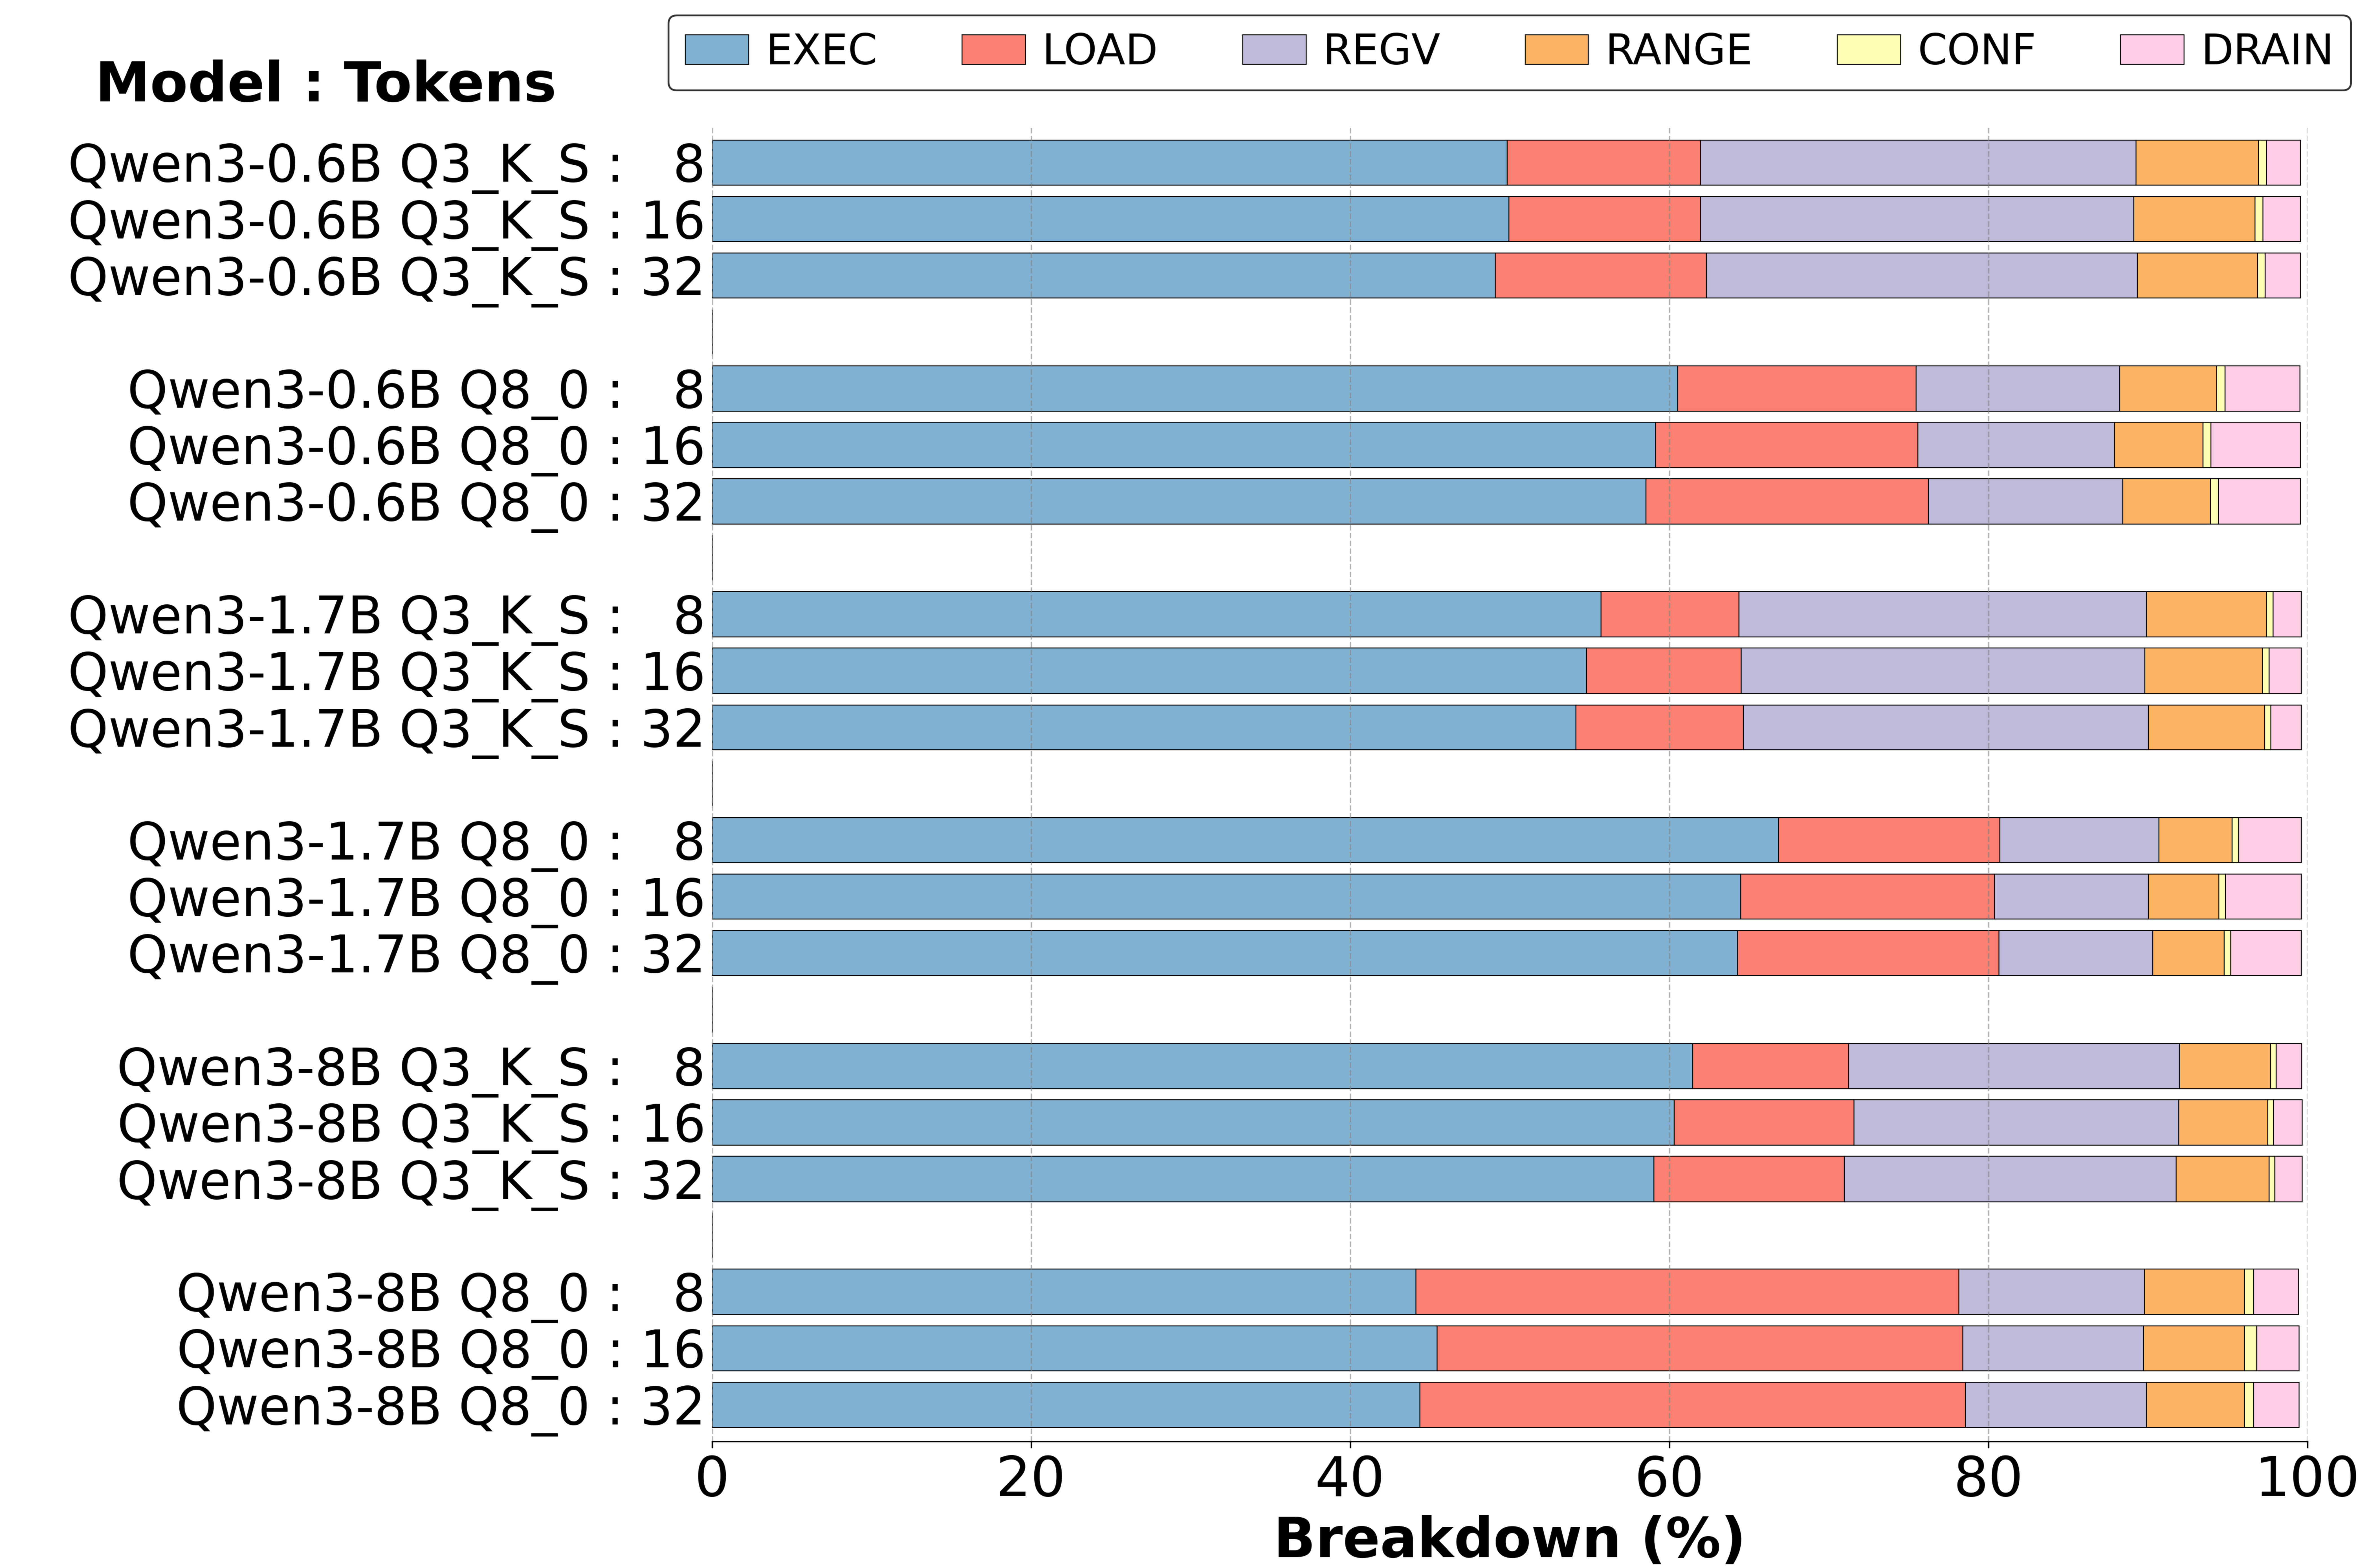
\includegraphics[width=\columnwidth]{./Prefill_breakdown_final.pdf}
  }\par\vspace{1em}
  \subfloat[Decode phase breakdown\label{fig:decode_breakdown}]{%
    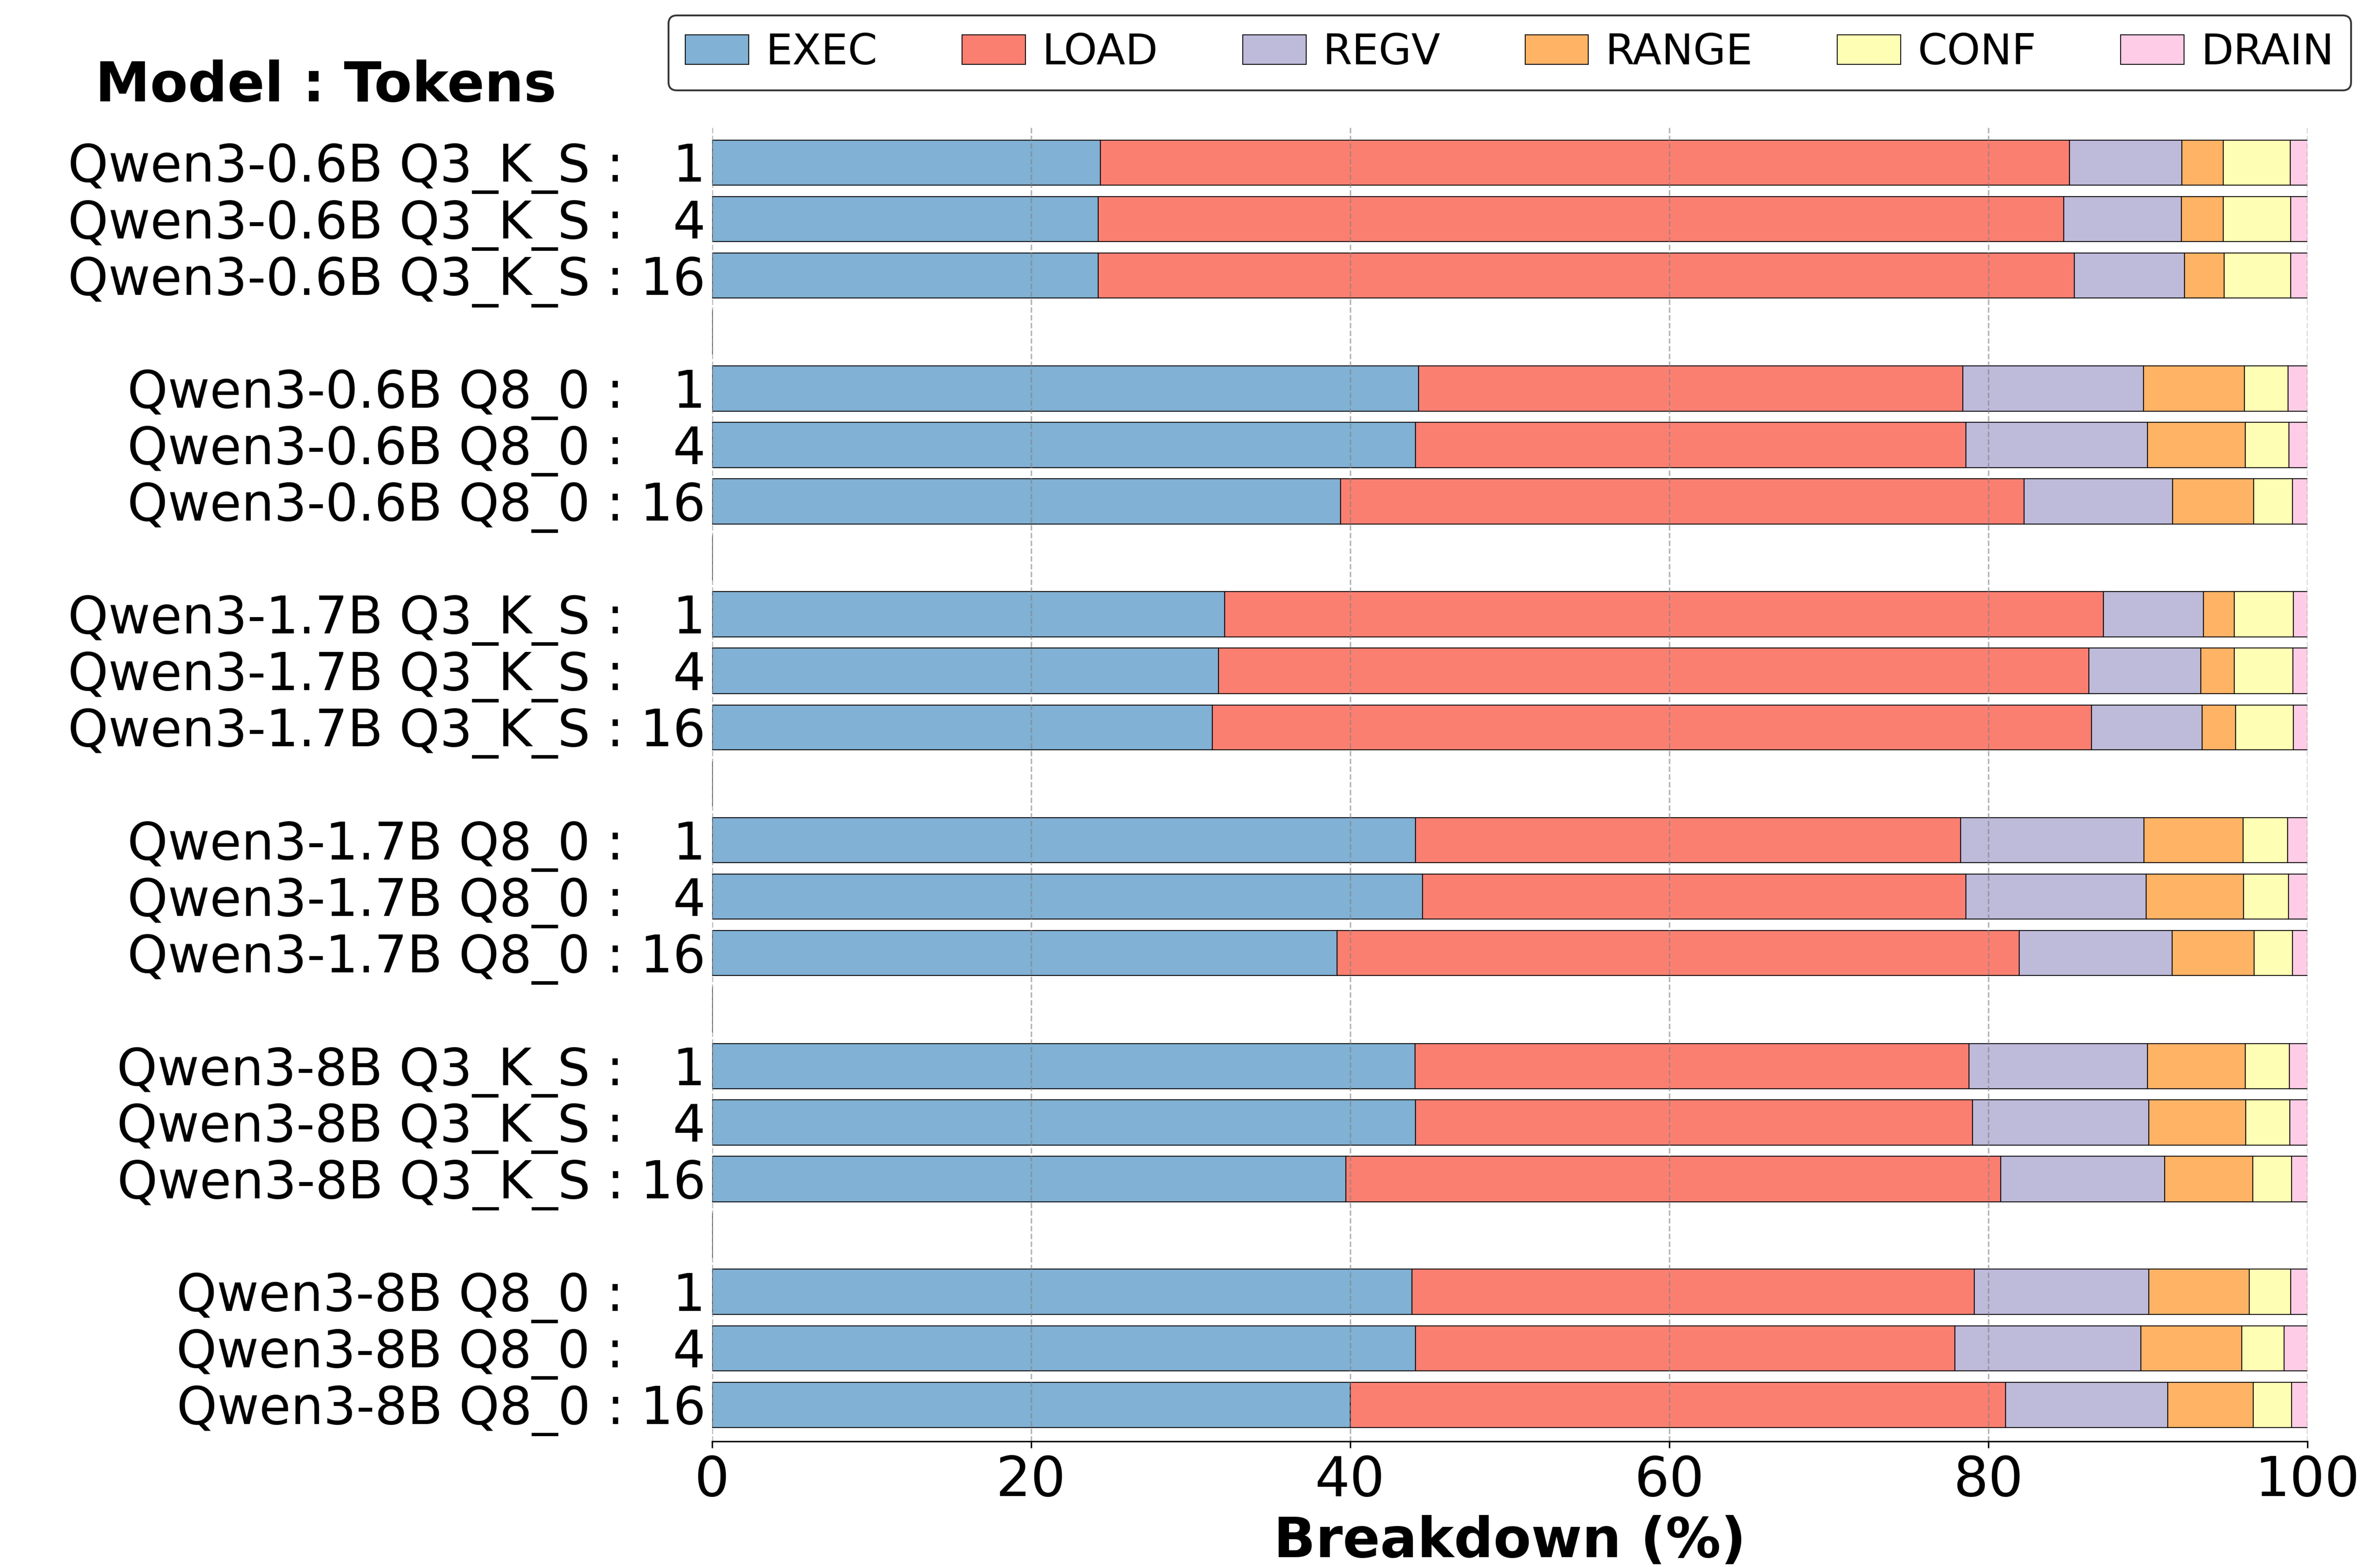
\includegraphics[width=\columnwidth]{./Decode_breakdown_final.pdf}
  }
  \caption{Breakdown of execution time within the IMAX accelerator for the Prefill and Decode phases.}
  \label{fig:execution_time_breakdown}
\end{figure}

\subsection{Analysis of IMAX Execution Time Breakdown}


To identify performance bottlenecks, we conducted a multi-level breakdown of the IMAX execution time. 
We first analyze the E2E latency from a system-level (macro) perspective, and then analyze the internal (micro) execution phases within the IMAX accelerator.

A detailed breakdown of the E2E latency for a representative workload (Qwen3-0.6B Q3\_K\_S with a [32:16] token I/O) reveals that system-level overheads are the dominant performance bottleneck. 
Out of a total latency of 16.3 s, the actual IMAX kernel execution accounted for only \SI{4.47}{\second} (\SI{27.4}{\percent}). 
The majority of the time was consumed by host CPU processing and DMA data loading from host to IMAX, which required \SI{5.43}{\second} (\SI{33.3}{\percent}) and \SI{5.31}{\second} (\SI{32.6}{\percent}), respectively. 
The remaining time was spent on DMA data drain (\SI{0.31}{\second}, \SI{1.9}{\percent}) and other IMAX configuration tasks (\SI{0.78}{\second}, \SI{4.8}{\percent}). 
This quantitative analysis immediately highlights a critical finding: the time spent on DMA data loading (\SI{5.31}{\second}) is substantial, exceeding even the net kernel execution time (\SI{4.47}{\second}).
While a degree of host CPU overhead (\SI{33.3}{\percent}) is expected in a heterogeneous system for tasks such as scheduling and data preparation, the significant latency from the DMA load points to the host-accelerator data path constitutes a definitive system-level bottleneck.


This system-level bottleneck is a direct reflection of the accelerator's internal behavior. 
To understand this relationship, we now analyze the breakdown of the time spent within the offloaded tasks on IMAX. 
LLM inference is characterized by two distinct phases: the prefill phase, which processes the input prompt in parallel, and the decode phase, which generates tokens sequentially. 
As shown in Fig.~\ref{fig:execution_time_breakdown}, we categorize the execution time of each phase into six components:
\begin{itemize}
  \item \textbf{EXEC}: Kernel execution time on the IMAX cores.
  \item \textbf{LOAD}: Duration of input data transfer from host main memory to the LMMs via DMA.
  \item \textbf{DRAIN}: Duration of result data transfer from the LMMs back to host main memory via DMA.
  \item \textbf{CONF}:  Host CPU overhead for configuring mapping commands on IMAX via Programmed I/O (PIO).
  \item \textbf{REGV}: Host CPU overhead for initializing internal Processing Element (PE) registers on IMAX via PIO.
  \item \textbf{RANGE}: Host CPU overhead for configuring the LMM address space on IMAX via PIO.
\end{itemize}



The prefill phase is generally compute-bound.
For most workloads, excluding the Qwen3-8B Q8\_0 model, the net computation time (EXEC) accounts for over \SI{50}{\percent} of the total execution time. 
This indicates that the computational resources of IMAX are being utilized efficiently. 
However, we also observe a trend where the proportion of time spent on data transfer~(LOAD) increases with the number of input tokens, a direct consequence of the larger data sizes associated with longer prompts. 
This suggests that even in the prefill phase, data transfer can become a significant bottleneck for large-scale models.
Furthermore, we note that the proportion of time spent on result data transfer~(DRAIN) is larger in the decode phase compared to the prefill phase. 
This difference in DRAIN ratio reflects the distinct data characteristics of each phase, specifically KV cache generation in prefill versus single token output in decode. 
This observation confirms that the behavior of the CGLA architecture aligns with the inherent workload duality.
While our experiments cover typical interactive scenarios, the performance implications for workloads with much longer token sequences, such as large document summarization, also warrant consideration. 
The trends observed suggest that data transfer would become an even more significant bottleneck in such scenarios. 
In the prefill phase, a longer prompt linearly increases the LOAD duration, while in the decode phase, a longer context length requires loading an ever-larger KV cache. 
These factors can lead to memory bandwidth saturation, indicating that the increasing data transfer overhead is a critical bottleneck for scaling to very long contexts. 
This observation suggests that enhancing the host-accelerator interconnect will be a key consideration for improving scalability in future architectural designs.

In contrast, the decode phase exhibits a clear memory-bound characteristic and is specifically LOAD-bound. 
This behavior stems from the algorithmic nature of the decode phase. 
The computational workload is relatively small, as only a single token is generated per step. 
However, the entire large KV cache, generated from all previous tokens, must be loaded from memory in each iteration.
The LOAD time is the primary component of the overall execution. 
Its proportional share grows with longer context lengths because of the corresponding expansion of the KV cache.
Finally, a notable observation in the prefill breakdown for the Q3\_K\_S models is the significant proportion of register initialization overhead~(REGV). 
This is primarily attributed to the Q6\_K kernel, which utilizes all 64 PEs of the IMAX architecture and thus requires a substantial amount of register configuration. 
The prefill phase's higher utilization of the Q6\_K kernel results in this increased REGV overhead.

These measurements were taken with IMAX's double-buffered LMMs actively overlapping computation and DMA transfers. 
That data transfer remains the dominant bottleneck, even with this hardware optimization, highlights the severity of the memory bandwidth challenge in LLM inference. 
While architectural overlap is essential, it is insufficient, indicating that further optimizations at both the system and algorithmic levels are required.


\begin{figure}[t]
  \centering
  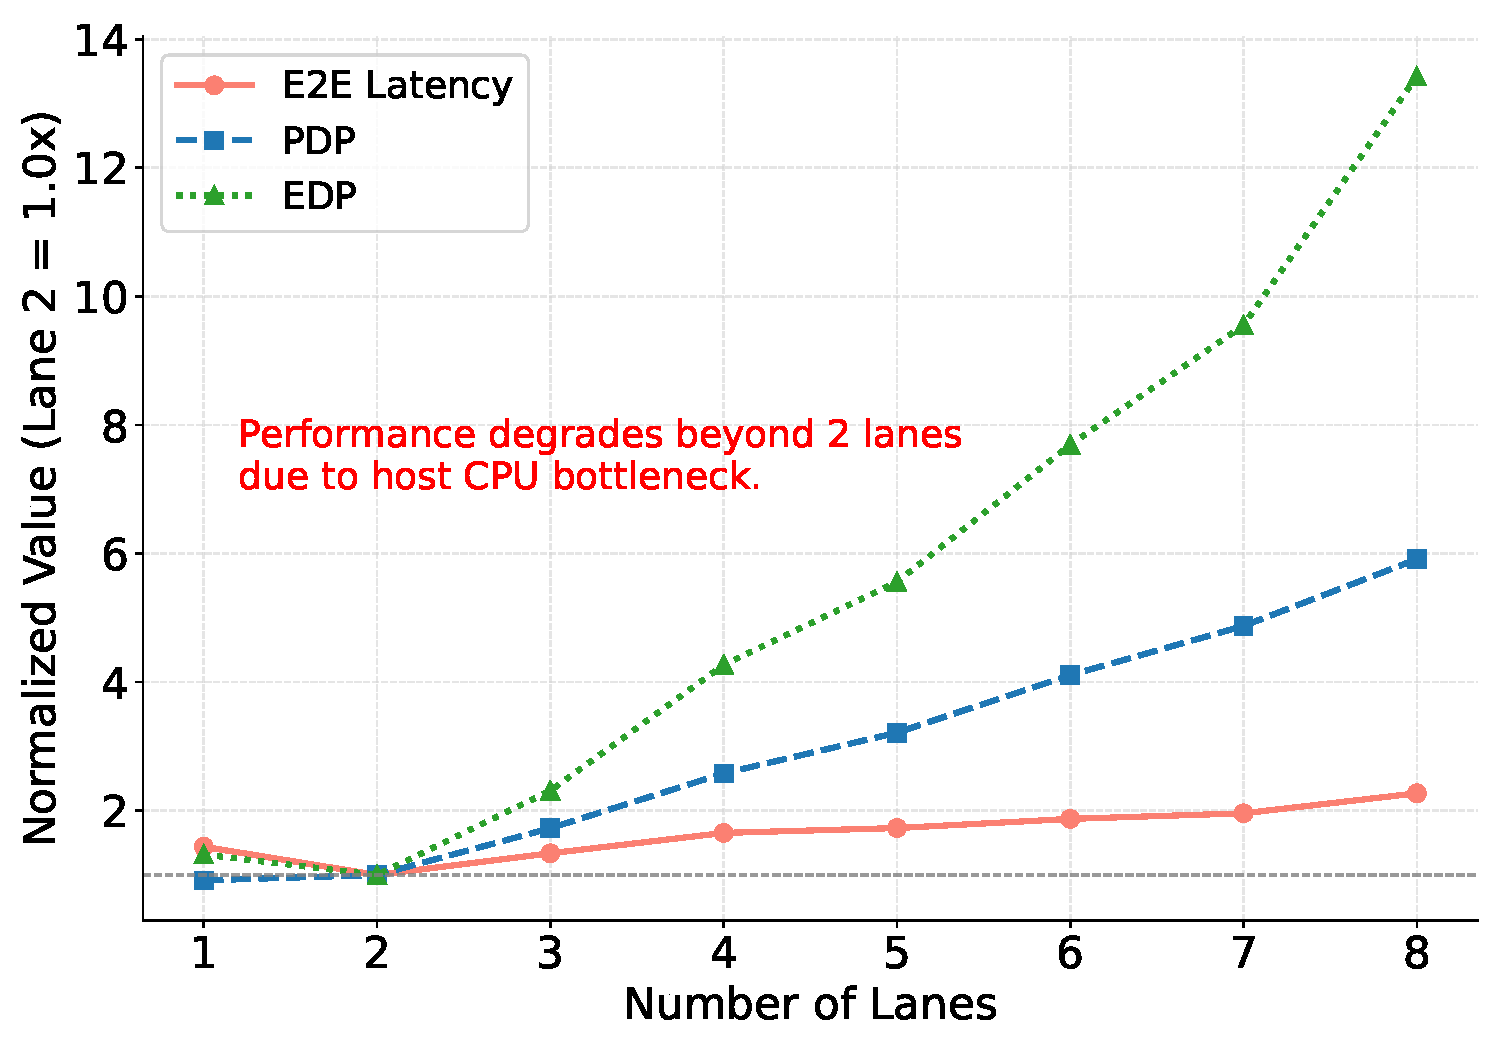
\includegraphics[width=1\columnwidth]{./performance_metrics_normalized.pdf}
  \caption{Scalability analysis of IMAX performance metrics as the number of compute lanes increases.}
  \label{fig:performance_metrics_normalized}

\end{figure}



\subsection{System-Level Limitations and Future Directions}
This work demonstrates the potential of a general-purpose CGRA for energy-efficient LLM inference, but it is equally important to discuss the limitations of our approach, which in turn define critical directions for future work.

A primary limitation, as revealed by our scalability analysis, is the architecture's dependence on the host system's performance.
As shown in Fig.~\ref{fig:performance_metrics_normalized}, performance saturates and then degrades beyond a two-lane configuration. 
This bottleneck is not inherent to the IMAX architecture itself but is a direct consequence of the dual-core ARM host's limited capability to manage data transfers and control flow for multiple parallel lanes. 
This finding highlights a fundamental challenge in heterogeneous computing, where an accelerator's performance is often constrained by its host system.
Therefore, a crucial next step is to integrate the IMAX architecture with a higher-performance host (e.g., an eight-core CPU), ideally via a high-bandwidth PCIe interconnect, to experimentally validate its true scalability potential.

Further limitations relate to the scope of our evaluation.
First, the performance and power figures for the \SI{28}{\nano\meter} ASIC are projections derived from synthesis tools. 
While based on standard industry practice, these estimates are subject to variations in the final physical implementation and manufacturing process. 
Second, our experiments were conducted on a specific embedded platform (AMD Versal VPK180 FPGA). 
System dynamics, particularly data transfer overhead, may differ significantly in other environments, such as a server with a PCIe-based interconnect. 
Finally, our analysis focused on the Qwen3 model family. 
Although our approach theoretically supports larger model sizes, the prototype's limited DMA buffer size restricted our experiments to the current configurations.
While representative, future work should extend this evaluation to models with diverse architectures, such as MoE, to ensure broader applicability.


Addressing these limitations forms a clear approach for future research. 
Beyond scaling the host system, optimizing the host-accelerator interface through software co-design and exploring hardware support for emerging low-bit quantization formats remain promising approaches to further enhance performance and efficiency.


